\documentclass[11pt]{article}
\usepackage[margin=1in, top=1in]{geometry}
\usepackage[all]{nowidow}
\usepackage[hyperfigures=true, hidelinks, pdfhighlight=/N]{hyperref}
\usepackage[separate-uncertainty=true, group-digits=false]{siunitx}
\usepackage{graphicx,amsmath,physics,tabto,float,amssymb,pgfplots,verbatim,tcolorbox}
\usepackage{listings,xcolor,subfig,caption,import,wrapfig,enumitem}
\usepackage[version=4]{mhchem}
\usepackage[noabbrev]{cleveref}
\newcommand{\creflastconjunction}{, and\nobreakspace}
\definecolor{stringcolor}{HTML}{C792EA}
\definecolor{codeblue}{HTML}{2162DB}
\definecolor{commentcolor}{HTML}{4A6E46}
\captionsetup{font=small, belowskip=0pt}
\lstdefinestyle{appendix}{
    basicstyle=\ttfamily\footnotesize,commentstyle=\color{commentcolor},keywordstyle=\color{codeblue},
    stringstyle=\color{stringcolor},showstringspaces=false,numbers=left,upquote=true,captionpos=t,
    abovecaptionskip=12pt,belowcaptionskip=12pt,language=Python,breaklines=true,frame=single}
\lstdefinestyle{inline}{
    basicstyle=\ttfamily\footnotesize,commentstyle=\color{commentcolor},keywordstyle=\color{codeblue},
    stringstyle=\color{stringcolor},showstringspaces=false,numbers=left,upquote=true,frame=tb,
    captionpos=b,language=Python}
\renewcommand{\lstlistingname}{Appendix}
\pgfplotsset{compat=1.17}

\begin{document}

\begin{center}
    \textbf{CP Tut 1}\hspace{2in}\textbf{KDSMIL001}\hspace{2in}\textbf{23-04-2022}
\end{center}

\begin{enumerate}
    \item \begin{enumerate}
        \item Using the method outlined on page 33 of the notes, we were able to simulate the decay of $N$ nuclei with an activity of $\Lambda=\SI{1.2}{\per\second}$. Running that simulation a number of times and noting how many decays occurred in each counting interval, for both 10s and 1s counting intervals, we were able to produce the plots in \cref{fig:q1ai,fig:q1aii}. Both times the simulation was run 1000 times.
        
        The means were found to be 1.205 with standard deviation 1.109 for \SI{1}{\second} and 11.243 with standard deviation 3.038 for \SI{10}{\second}. The expected mean is $\Lambda T$ where $T$ is the counting interval so with their respective standard deviations, they are reasonably close to the expected value.
        
        \begin{figure}[h]
            \begin{center}
                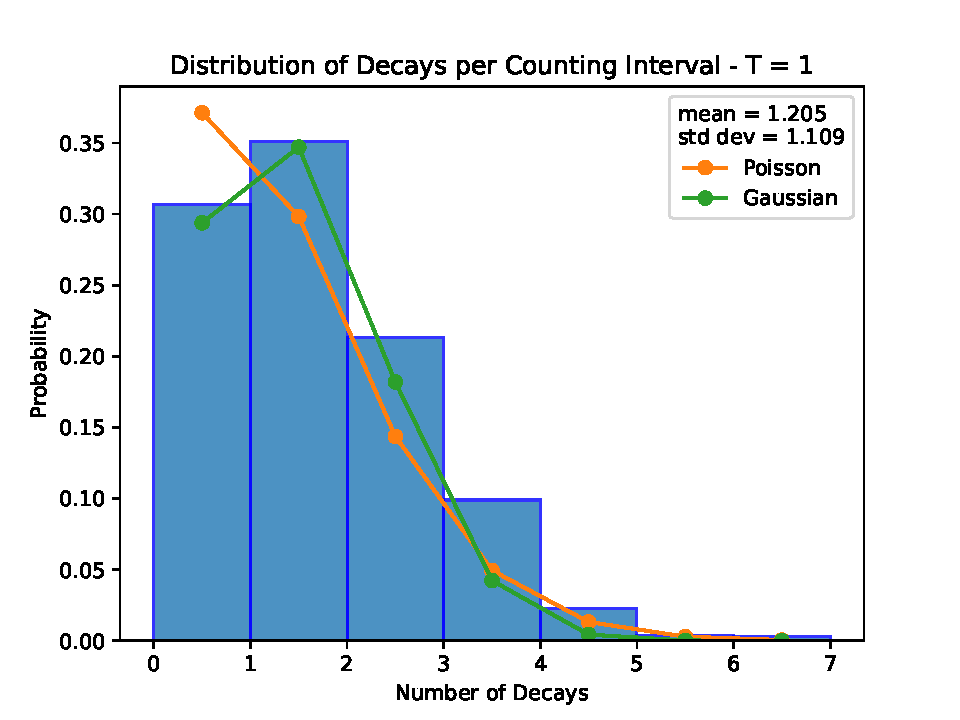
\includegraphics[width=0.6\textwidth]{Plots/q1ai.pdf}
                \caption{Distribution of decays per counting interval for $T=\SI{1}{\second}$, normalised and plotted with the Poisson and Gaussian distributions of the same mean and standard deviation. Simulation run 1000 times.}
                \label{fig:q1ai}
            \end{center}
        \end{figure}
        
        \begin{figure}[h]
            \begin{center}
                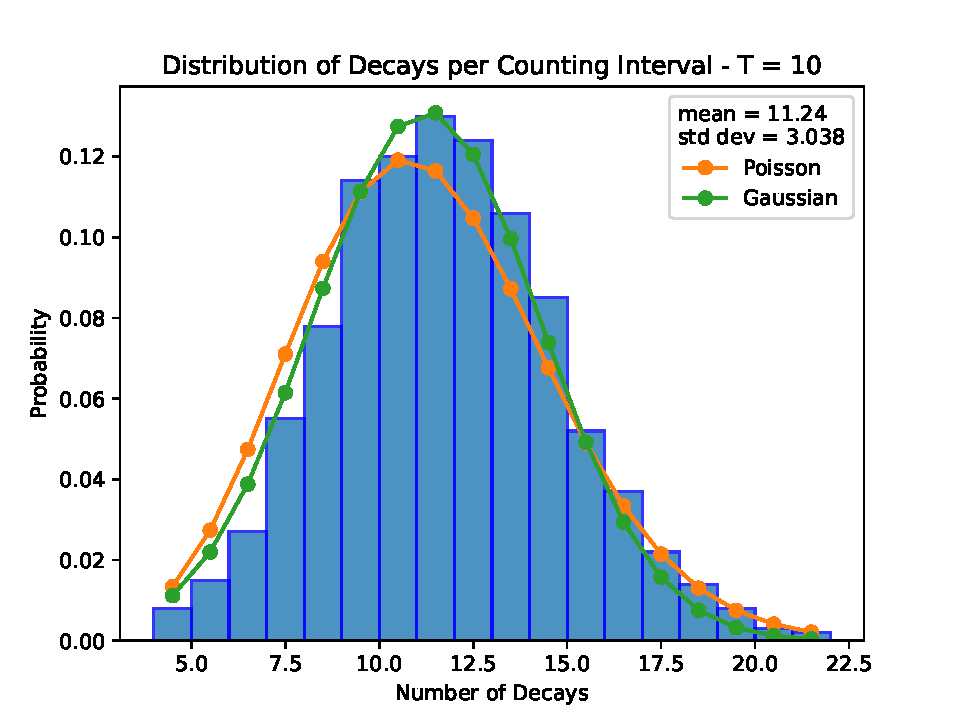
\includegraphics[width=0.6\textwidth]{Plots/q1aii.pdf}
                \caption{Distribution of decays per counting interval for $T=\SI{10}{\second}$, normalised and plotted with the Poisson and Gaussian distributions of the same mean and standard deviation. Simulation run 1000 times.}
                \label{fig:q1aii}
            \end{center}
        \end{figure}

        \item Along with the results of 1. a), \cref{fig:q1ai,fig:q1aii} show the comparison between the histograms and both a Poisson distribution as well as a Gaussian distribution. The mean used to plot both, as well as the standard deviation for the Gaussian, was drawn from the data itself. 
        
        We can see in both cases that the data is best modelled by the Gaussian distribution, which is not what we expect. For such low means, we expect the Poisson distribution to not be modelled well by the Gaussian, and we expect the data to follow a Poissonian distribution. The standard deviation of the data seems to suggest a Poissonian distribution, as both are close the the square root of the mean, but the plots suggest otherwise.

        \item In order to investigate the distribution of times between successive decays of the nuclei, we chose a counting interval of \SI{10}{\second} and ran the simulation 1000 times. Each time a decay occurred, the current time in the simulation was noted and if no decays had happened in the time step, the time since the last decay was calculated and added to an array. If there had already been a decay in that time step, the decay was ignored in order to avoid an interval of 0 seconds. The distribution resulting from this analysis, along with the expected form of an exponential distribution, is shown in \cref{fig:q1c}. 
        
        In order to work out the expected mean, we can think about $\Lambda$ telling us that we expect, on average, 1.2 decays every second, so the time between decays should be $1/\Lambda$, or \SI{0.833}{\second}. Looking at the mean in \cref{fig:q1c}, we find it to be \SI{0.801}{\second}. Throughout all our testing it was consistently lower than expected. We are not sure why this is.

        \begin{figure}[h]
            \begin{center}
                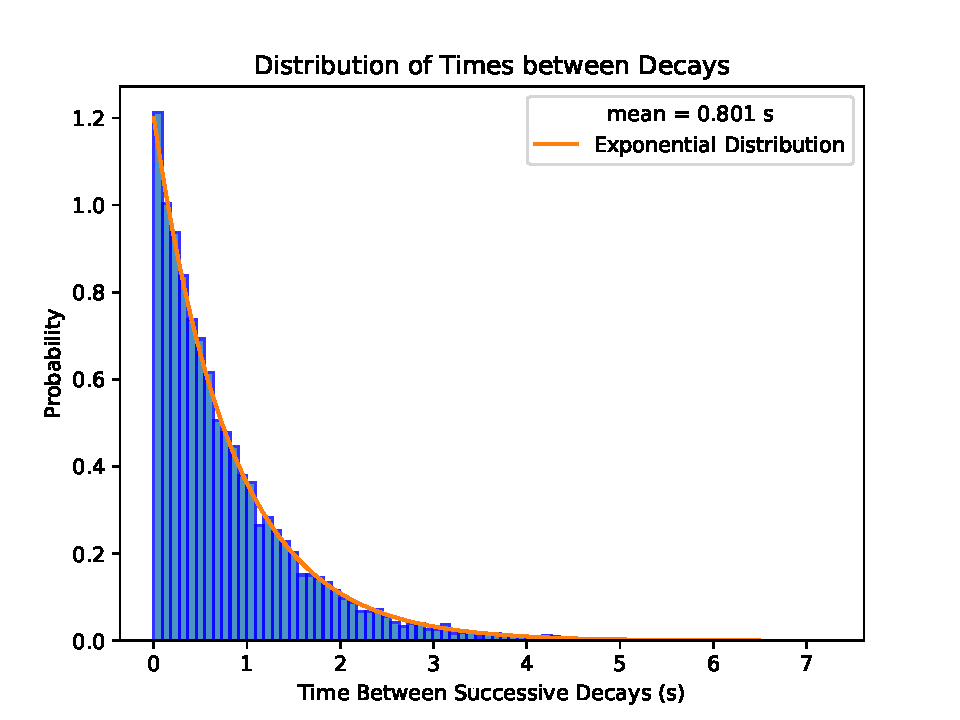
\includegraphics[width=0.6\textwidth]{Plots/q1c.pdf}
                \caption{Distribution of times between successive decays, ignoring decays that happen in the same time step. Plotted with the histogram is the exponential distribution with $\lambda=\Lambda$, the activity.}
                \label{fig:q1c}
            \end{center}
        \end{figure}
    \end{enumerate}

    \item \begin{enumerate}
        \item In order to use the transformation method, we integrated each probability distribution and rearranged to find $y_i$ in terms of the uniformly distributed $x_i$:
        \begin{enumerate}[label=\roman*)]
            \item \label{itm:q2ai}
            \begin{align*}
                x_i &=\int_{-\frac{\pi}{4}}^{y_i}\cos(2y')dy'\\
                &=\frac 12 (\sin(2y_i)+1)\\
                \implies y_i&=\frac{1}{2}\arcsin(2x_i-1)
            \end{align*}

            \item \label{itm:q2aii}
            \begin{align*}
                x_i&=\int_2^{y_i}\frac{1}{\sqrt 8 - \sqrt 3}\frac{y'}{\sqrt{y'^2-1}}dy'\\
                &=\frac{1}{\sqrt 8 - \sqrt 3}\left(\sqrt{y_i^2-1}-\sqrt 3\right)\\
                \implies y_i&=\sqrt{(x_i(\sqrt{8}-\sqrt{3})+\sqrt{3})^2+1}
            \end{align*}

            \item \label{itm:q2aiii}
            \begin{align*}
                x_i&=\int_1^{y_i}\frac{1}{\sqrt 8}\frac{y'}{\sqrt{y'^2-1}}dy'\\
                &=\sqrt{\frac{y_i^2-1}{8}}\\
                \implies y_i&=\sqrt{8x_i^2+1}
            \end{align*}
        \end{enumerate}
        Then by simply generating 500 000 random numbers in $[0,1)$ and feeding them through the equations found above, we could generate 500 000 numbers distributed according to the respective probability distribution.

        \begin{figure}[H]%
            \centering
            \subfloat[\centering Uniform distribution of $x_i$ values]{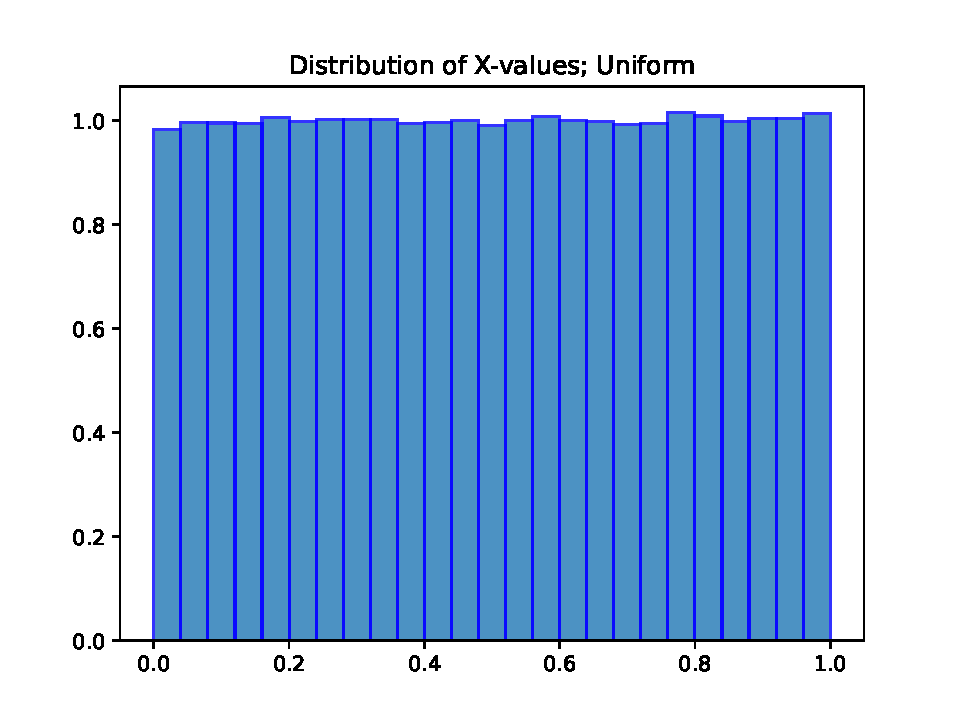
\includegraphics[width=.45\textwidth]{Plots/q2aix.pdf}}
            \,
            \subfloat[\centering Distribution of $y_i$ values]{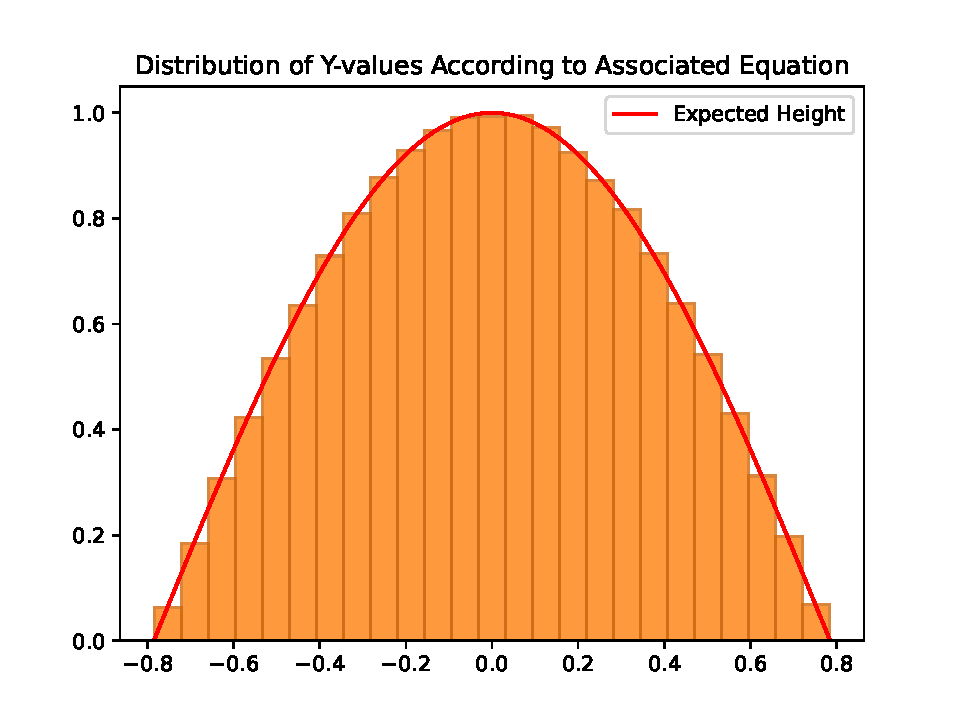
\includegraphics[width=.45\textwidth]{Plots/q2aiy.pdf}}
            \caption{The uniform distribution of numbers in $[0,1)$ alongside the $y_i$ values generated from them using the transformation method, according to $p(y)=\cos(2y)$. Plotted with the transformed distribution is the expected probability distribution. Each distribution is split into 25 bins of equal width. 500 000 numbers were generated. Both the histogram and the expected form are normalised to be a pdf.}
            \label{fig:q2ai}
        \end{figure}

        \begin{figure}[H]%
            \centering
            \subfloat[\centering Uniform distribution of $x_i$ values]{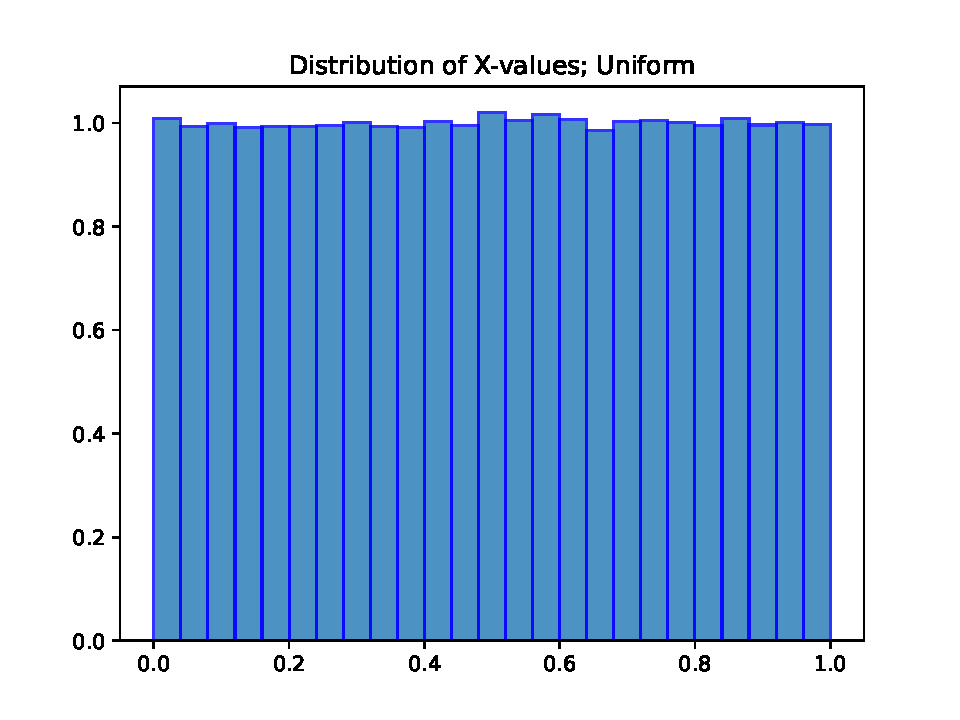
\includegraphics[width=.45\textwidth]{Plots/q2aiix.pdf}}
            \,
            \subfloat[\centering Distribution of $y_i$ values]{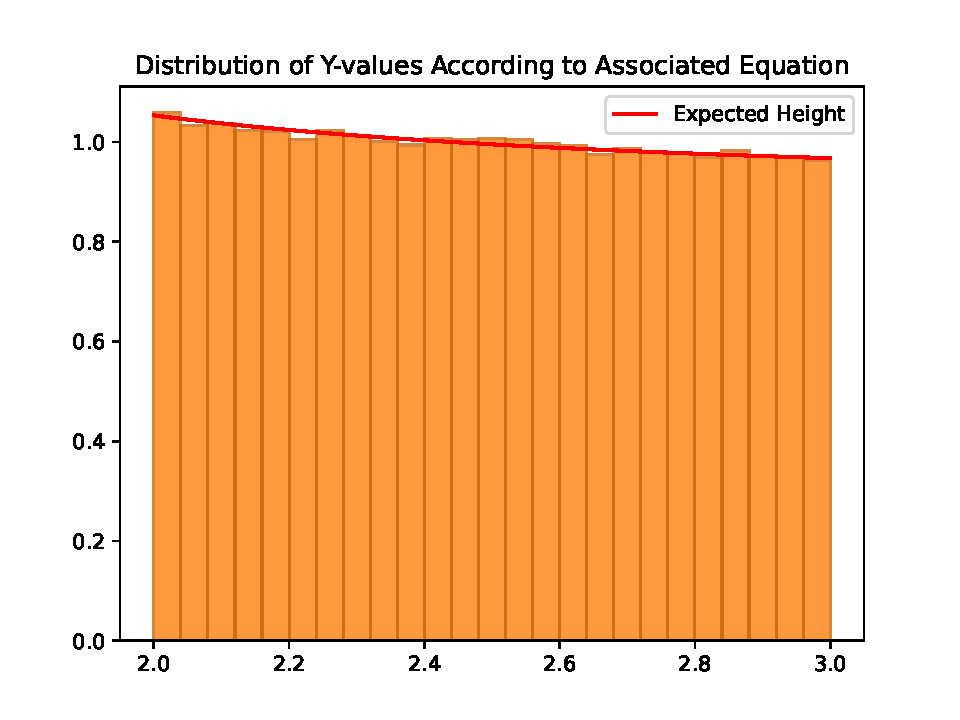
\includegraphics[width=.45\textwidth]{Plots/q2aiiy.pdf}}
            \caption{The uniform distribution of numbers in $[0,1)$ alongside the $y_i$ values generated from them using the transformation method, according to $p(y)=\frac{1}{\sqrt 8 - \sqrt 3}\frac{y}{\sqrt{y^2-1}}$. Plotted with the transformed distribution is the expected probability distribution. Each distribution is split into 25 bins of equal width. 500 000 numbers were generated. Both the histogram and the expected form are normalised to be a pdf.}
            \label{fig:q2aii}
        \end{figure}

        \begin{figure}[H]%
            \centering
            \subfloat[\centering Uniform distribution of $x_i$ values]{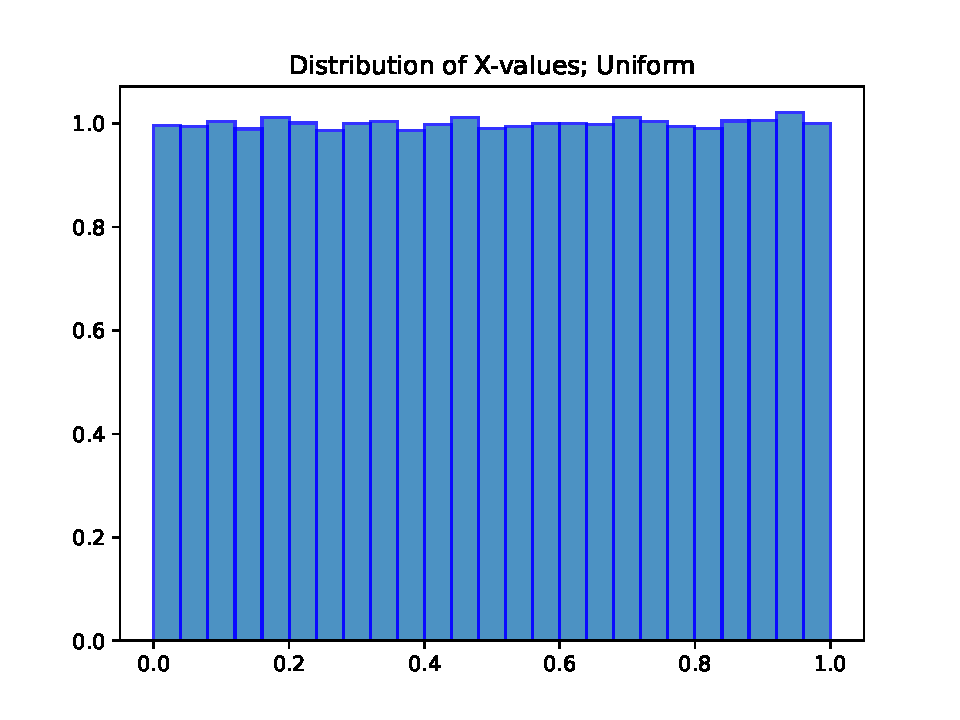
\includegraphics[width=.45\textwidth]{Plots/q2aiiix.pdf}}
            \,
            \subfloat[\centering Distribution of $y_i$ values]{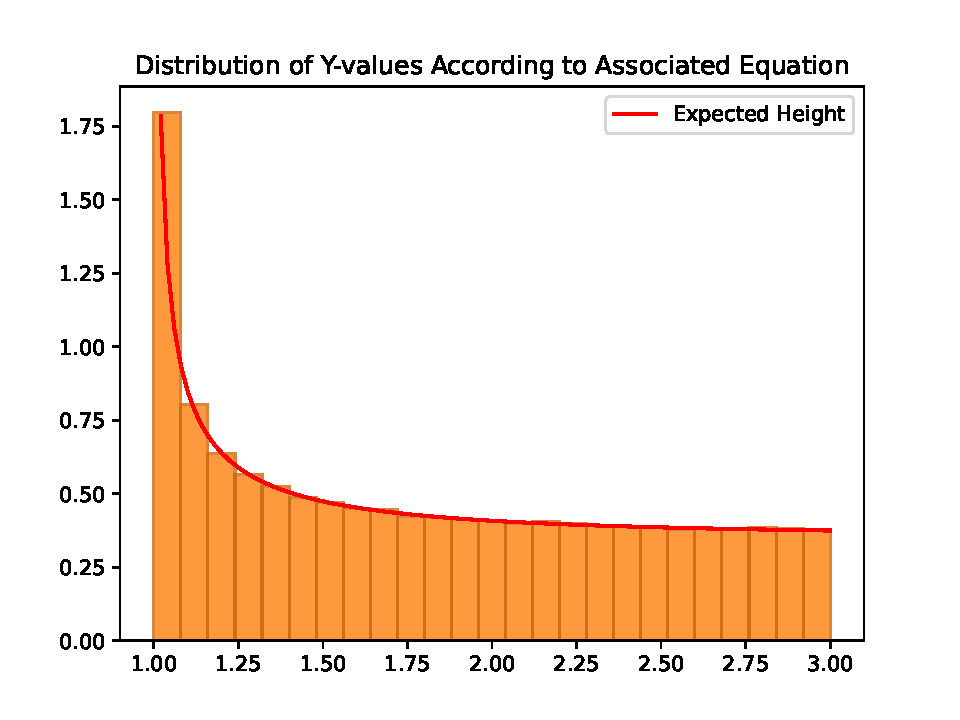
\includegraphics[width=.45\textwidth]{Plots/q2aiiiy.pdf}}
            \caption{The uniform distribution of numbers in $[0,1)$ alongside the $y_i$ values generated from them using the transformation method, according to $p(y)=\frac{1}{\sqrt 8}\frac{y}{\sqrt{y^2-1}}$. Plotted with the transformed distribution is the expected probability distribution. Each distribution is split into 25 bins of equal width. 500 000 numbers were generated. Both the histogram and the expected form are normalised to be a pdf.}
            \label{fig:q2aiii}
        \end{figure}

        We can see in each case that the transformation method worked well, accurately approximating the respective probability distribution. 

        \item Next, we aimed to use the rejection method to generate 500 000 random numbers according to the distribution in \cref{fig:q2ai}: $p(y)=\cos(2y)$. To do this we first find the maximum value of $p(y)$ in the interval of interest, then generate a pair of numbers corresponding to a coordinate in the box bounded by the interval and the maximum value. If this coordinate falls within the distribution, it is accepted, otherwise it is rejected and we try again. This is repeated until the required amount of numbers $y_i$ are generated, in our case 500 000. 
        
        In order to speed up computation, we wanted to avoid generating a random number at each iteration, so a set of random numbers is generated at the start and then looped over to find those that will be accepted. This requires knowing how many, on average, will be accepted by the algorithm. This can be calculated using
        \begin{equation}
            P(\text{accept}) = \frac{\int_a^b p(y) dy}{p_{\text{max}}(b-a)}=\frac{1}{p_{\text{max}}(b-a)}
        \end{equation}
        The last step assumes the probability distribution is normalised. With this, we can generate $NP(\text{accept})$ random numbers, multiplied by 1.5 to be safe, and be certain that we will accept at least $N$ in the process.

        Using this method, we produced the plot in \cref{fig:q2b}, finding that the method approximated the true distribution fairly well. 

        \begin{figure}[h]
            \begin{center}
                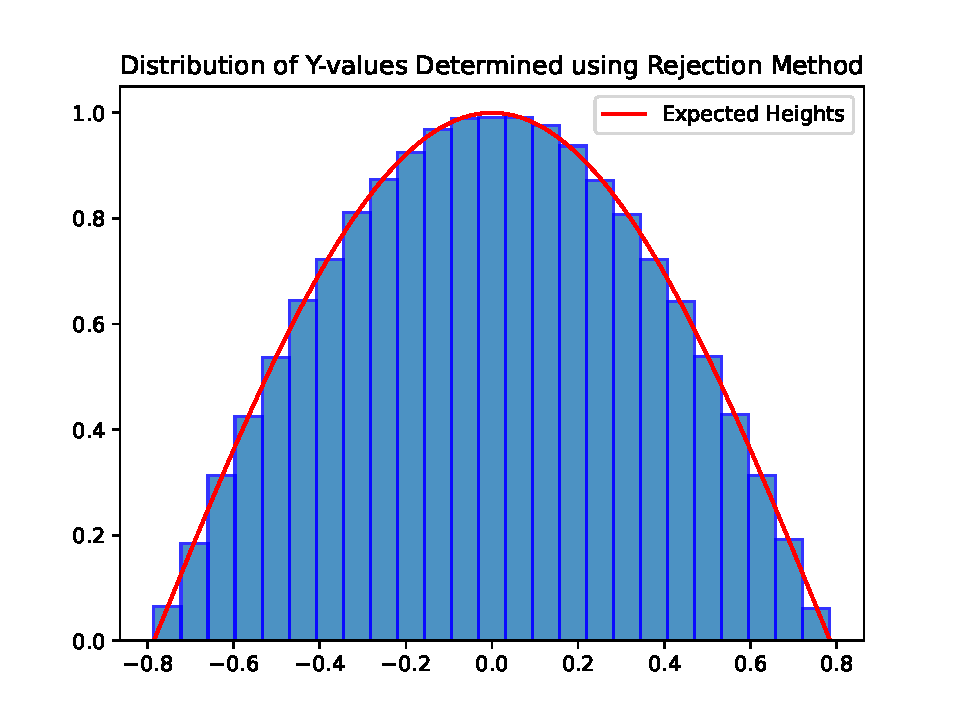
\includegraphics[width=.6\textwidth]{Plots/q2b.pdf}
                \caption{Random numbers distributed according to $p(y)=\cos(2y)$ using the rejection method. 500 000 numbers were generated. The data is histogrammed into 25 bins of equal width. The expected form of the distribution is plotted along with the histogram. Both the histogram and the expected form are normalised to be a pdf.}
                \label{fig:q2b}
            \end{center}
        \end{figure}
        
        \item The rejection method could be used to generate the distribution in \cref{itm:q2aii} as it is fairly flat and as such would have a relatively high acceptance rate. On the other hand, \cref{itm:q2aiii} would not be able to be generated using rejection, at least not easily. It blows up at $y=1$ and as such would have a maximum in the interval of $\infty$. This would effectively make the acceptance rate 0. Even ignoring that end of the interval wouldn't help as near to it the value of the distribution would still be very large, leading to a low acceptance rate.
    \end{enumerate}

    \item The probability distribution to generate numbers according to was
    
    \begin{equation}
        p(y)=\frac{1}{4.6997309}\frac{\sin^2(y)+1}{y^{4/3}},\;\;\;y\in(1,+\infty)
        \label{eqn:q3eqn}
    \end{equation}

    The implementation of the rejection method in this case is practically identical to the previous case. It has an acceptance probability of about $p(\text{accept})=0.0278$, so close to 50 million random pairs had to be generated in order to ensure we had 1 000 000 numbers at the end. This is obviously computationally very costly. We also had to cut the function at some upper bound as $+\infty$ is too large. $y=100$ was chosen. The results are in \cref{fig:q3rejection}.
    
    \begin{figure}[h]
        \begin{center}
            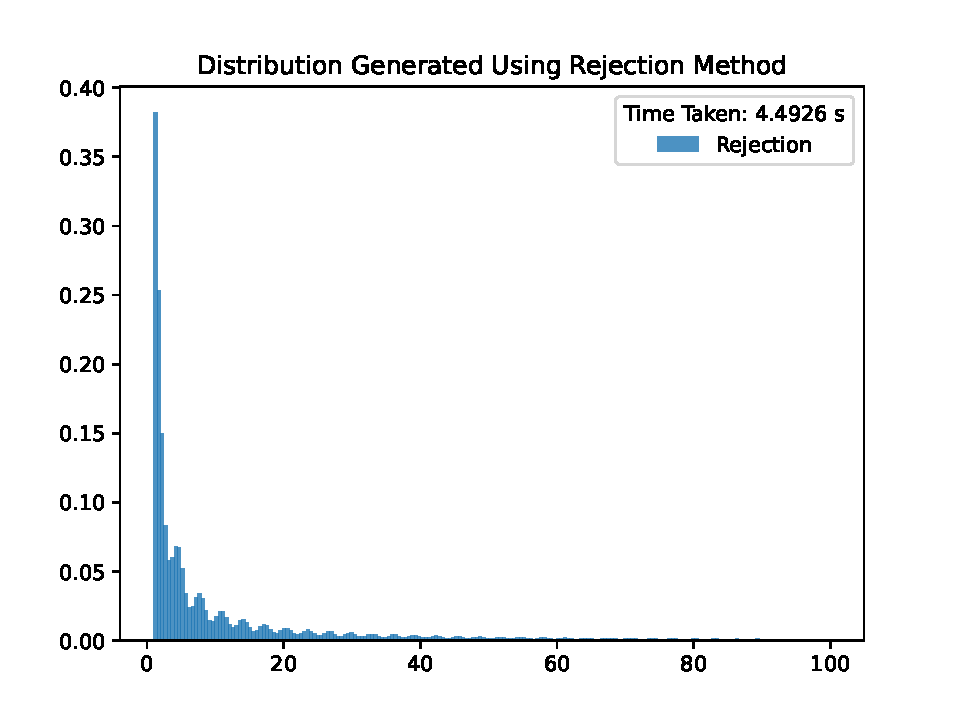
\includegraphics[width=.6\textwidth]{Plots/q3rejection.pdf}
            \caption{Normalised histogram of 1 000 000 random numbers generated according to \cref{eqn:q3eqn} using the rejection method on the interval $[1,100]$. This took \SI{4.4926}{\second} to complete. The histogram is split into 200 bins of equal width.}
            \label{fig:q3rejection}
        \end{center}
    \end{figure}

    The combination method was also implemented to generate numbers according to \cref{eqn:q3eqn}. The acceptance rate is given by

    \begin{equation}
        p(\text{accept})=\frac{\int_a^b p(y) dy}{\int_a^b Cf(y) dy}
        \label{eqn:q3acceptance}
    \end{equation}

    where $f(y)$ is a function for which we can generate a distribution using the transformation method, that resembles the distribution $p(y)$, and $C$ is a scaling factor such that $p(y)\leq Cf(y)$ for all $y\in[a,b]$. We chose this $f(y)$ to be 

    \begin{equation}
        f(y)=\frac{1}{3y^{4/3}}
        \label{eqn:q3f}
    \end{equation}

    and $C=6/4.997309$. Using this acceptance rate, which we found to be about 0.788, we generated enough random pairs such that we ended up with 1 000 000 random numbers distributed according to \cref{eqn:q3eqn}. This method is able to generate numbers over infinite and semi-infinite intervals, such as this one. That was done in this case but for the sake of comparison we restricted the interval to $[1,100]$. The results are in \cref{fig:q3combo}.

    \begin{figure}[h]
        \begin{center}
            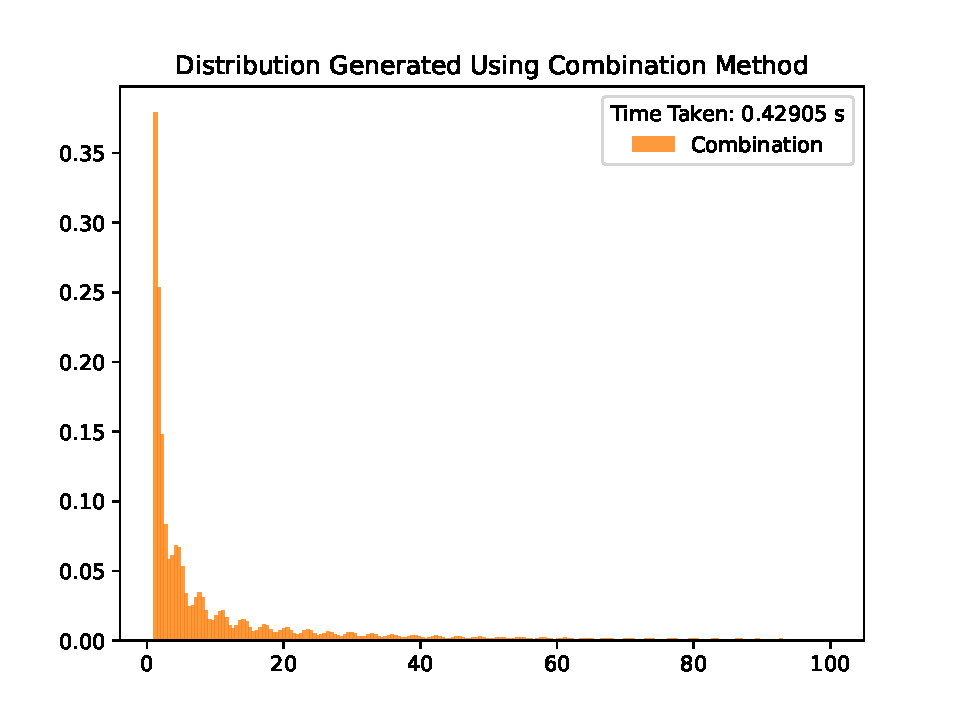
\includegraphics[width=.6\textwidth]{Plots/q3combo.pdf}
            \caption{Normalised histogram of 1 000 000 random numbers generated according to \cref{eqn:q3eqn} using the combination rejection-transformation method on the interval $[1,100]$. This took \SI{0.428}{\second} to complete. The histogram is split into 200 bins of equal width.}
            \label{fig:q3combo}
        \end{center}
    \end{figure}

    We can see that the combination method is about 10 times faster than the rejection method. This makes sense when we consider that the acceptance rate of the combination method is so much larger than that for rejection method, meaning far fewer random numbers needed to be generated at the start for the combination method. Other than the generation of the numbers the methods perform pretty much the same operations, so this difference in time taken is most likely all due to that.\\
    Since the combination method produces numbers on the entire interval, not just $[1,100]$, we had to exclude some values when plotting \cref{fig:q3combo}. That number turned out to be 205 949 of the 1 000 000 values generated. Because of this number that get excluded, roughly $1/5$ of the total, the histograms for the combination method are naturally lower than those of the rejection method, as can be seen in \cref{fig:q3comparison}.

    \begin{figure}[h]
        \begin{center}
            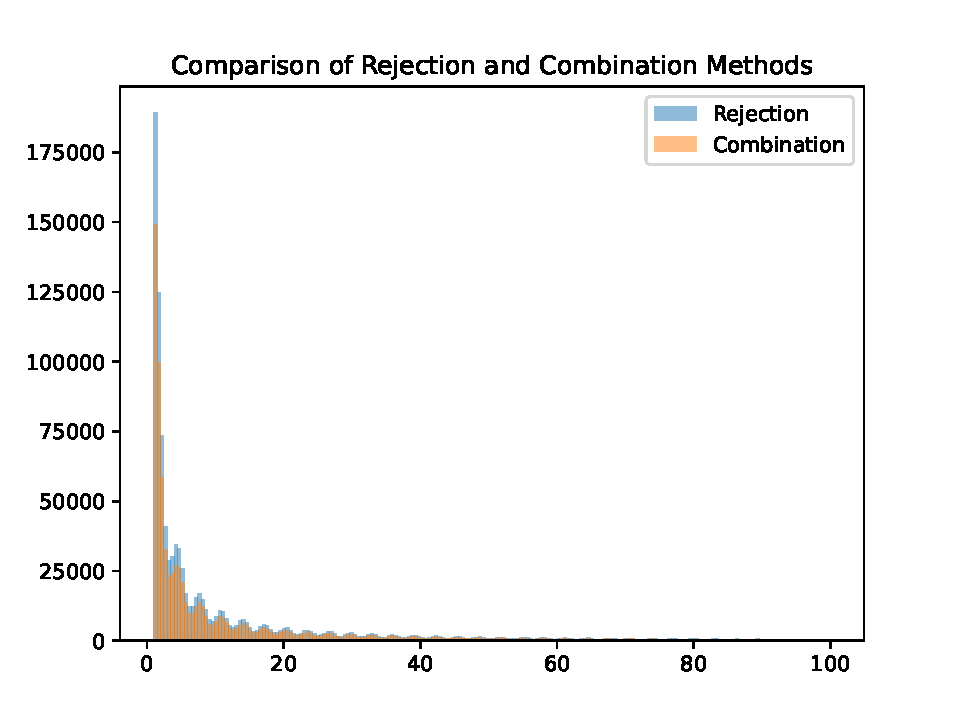
\includegraphics[width=.6\textwidth]{Plots/q3comparison.pdf}
            \caption{Comparison of the un-normalised distributions generated using the rejection and comparison methods. Note that the comparison method produces consistently lower histograms.}
            \label{fig:q3comparison}
        \end{center}
    \end{figure}
    

    \item \begin{enumerate}
        \item \begin{enumerate}
            \item If $\Delta$ is small, there is a high chance that the probability at that position is very similar to that at the current position, so there's a high chance that the trial position will be accepted. With a large $\Delta$, the trial position could be all over the place, so there is less likely to be acceptance, but we are more likely to sample the entire space, thus leading to faster equilibration.
            \item Using $\sigma=1$, we plotted the ratio of accepted values to total iterations as a function of $\Delta$, and picked a value of the ratio of around 0.4, leading to a choice of $\Delta=4$. \\
            Finding the equilibration time proved a difficult task, giving inconsistent results.
        \end{enumerate}
        
        \item The asymptotic distribution is of course expected to be the form of a Gaussian, and using 100 000 points we find the distribution in \cref{fig:q4b}, which very closely resembles a Gaussian distribution with the intended mean and standard deviation ($\langle x \rangle=0,\;\sigma=1$). The mean and standard deviation of the generated distribution were found to be ($\langle x \rangle=0.00647,\;\sigma=1.00098$ after 100 000 iterations.
        
        \begin{figure}[h]
            \begin{center}
                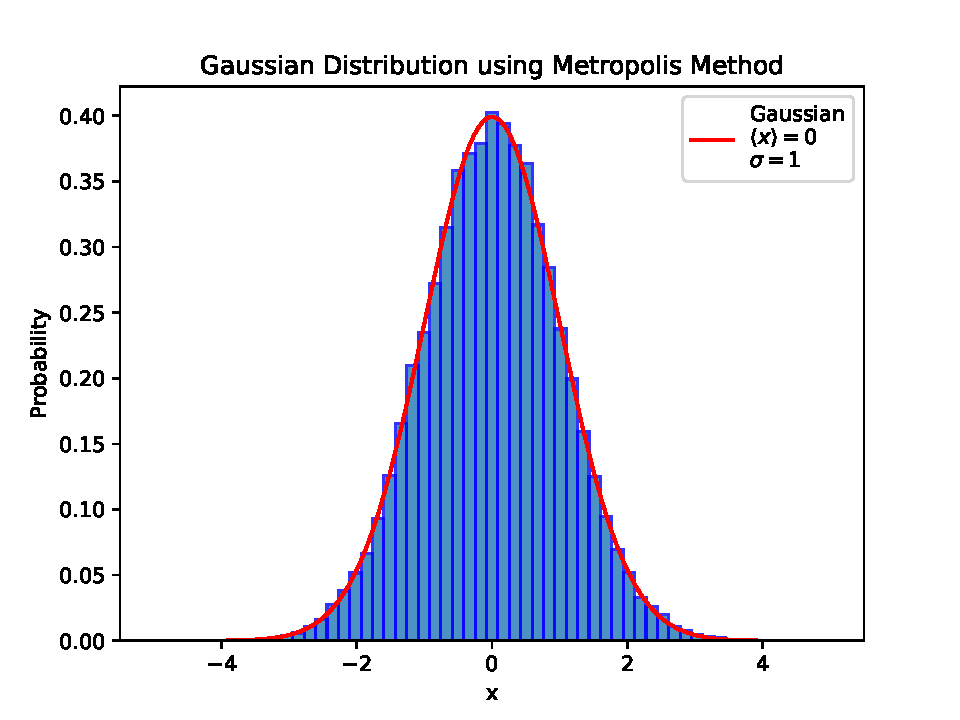
\includegraphics[width=.6\textwidth]{Plots/q4b.pdf}
                \caption{Asymptotic distribution of numbers generated using the Metropolis Method according to a Gaussian Distribution. 100 000 iterations were performed, with an acceptance ratio of 0.39289. Plotted with the normalised histogram is the expected Gaussian distribution with $\langle x \rangle=0,\;\sigma=1$. }
                \label{fig:q4b}
            \end{center}
        \end{figure}

        \item \begin{enumerate}
            \item For a value of $j=0$, the autocorrelation function is calculating the correlation of a value with itself, so we expect that there is complete correlation, i.e. $C(j=0)=1$.
            \item If $x_i$ were completely random, there should be no correlation between any of the values in the distribution, so for $j\neq 0$, we would expect $C=0$.
            \item For our distribution generated in b), we calculated the correlation function for $j\neq 0$ and when it came within some distance of 0, we stopped. We chose this distance to be \num{1e-3} and the autocorrelation function came to within that distance of 0 first for $j=29$. A plot of autocorrelation with respect to $j$ is shown in \cref{fig:q4c}.
            
            \begin{figure}[h]
                \begin{center}
                    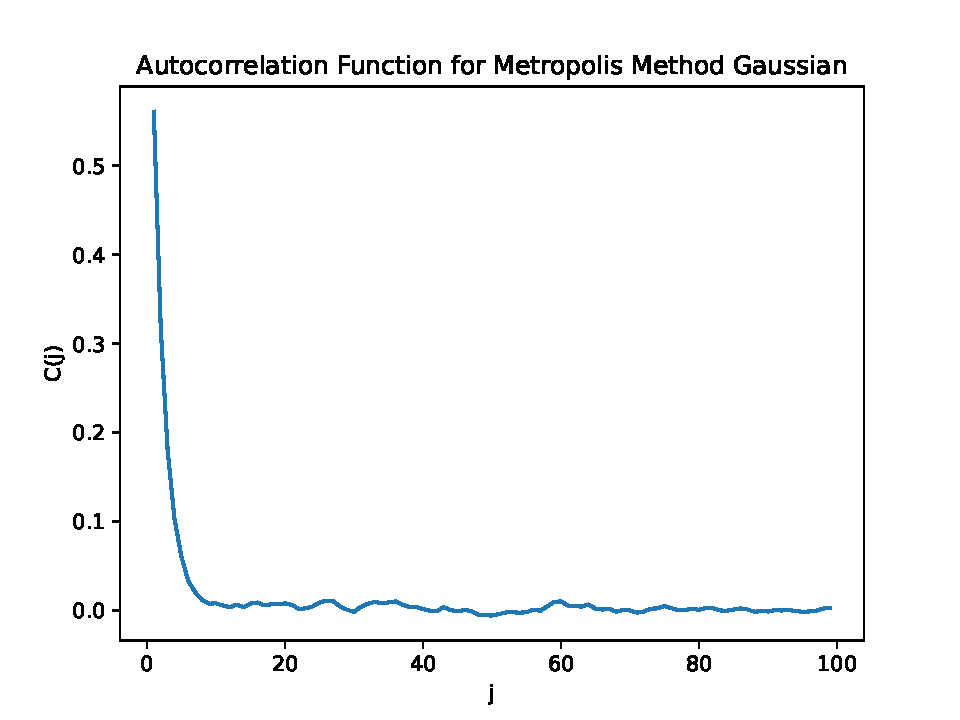
\includegraphics[width=.6\textwidth]{Plots/q4c.pdf}
                    \caption{Plot of the autocorrelation function of the Gaussian distribution produced using the Metropolis Method. $C(j)$ falls below \num{1e-3} after 29 steps.}
                    \label{fig:q4c}
                \end{center}
            \end{figure}
        \end{enumerate}
    \end{enumerate}
\end{enumerate}

% q3 results
% pHit: 0.027792733488535566
% rejectionRate 0.788316
% rejection average: 12.458407178501192
% combo average: 12.48345169474772
% number of combo above 100: 205949
% Time taken for Rejection Method: 4.492590665817261
% Time taken for Combination Method: 0.4290454387664795

\end{document}